%==============================================================================
% Sjabloon poster bachproef
%==============================================================================
% Gebaseerd op document class `a0poster' door Gerlinde Kettl en Matthias Weiser
% Aangepast voor gebruik aan HOGENT door Jens Buysse en Bert Van Vreckem

\documentclass[a0,portrait]{hogent-poster}

% Info over de opleiding
\course{Bachelorproef}
\studyprogramme{toegepaste informatica}
\academicyear{2024-2025}
\institution{Hogeschool Gent, Valentin Vaerwyckweg 1, 9000 Gent}

% Info over de bachelorproef
\title{Stemmen onderscheiden voor het opsporen van elderspeak in de Vlaamse zorgcontext}
%\subtitle{Ondertitel (eventueel)}
\author{Lisa Verhoeyen}
\email{lisa.verhoeyen@student.hogent.be}
\supervisor{Veerle Depestele}
\cosupervisor{Jorrit Campens (HOGENT)}

% Indien ingevuld, wordt deze informatie toegevoegd aan het einde van de
% abstract. Zet in commentaar als je dit niet wilt.
\specialisation{AI \& Data Engineering}
\keywords{speaker diarization, stemmen onderscheiden, elderspeak}
\projectrepo{https://github.com/LisaVerhoeyen/bp-stemmen-onderscheiden}

\begin{document}

\maketitle

\begin{abstract}
Ondanks het feit dat de zorgsector de dag van vandaag vooral op persoonsgerichte zorgverlening focust, ervaren oudere patiënten vaak dat de communicatie te betuttelend is. Dit fenomeen staat bekend als elderspeak of secondary babytalk. Om dit tegen te gaan is er vanuit de opleiding verpleegkunde aan HOGENT het initiatief genomen om een applicatie te gebruiken die de studenten erop wijst dat ze gebruik maken van elderspeak. Deze applicatie werd reeds ontworpen in voorgaande bachelorproeven aan HOGENT, maar er ontbreken nog een aantal functionaliteiten voordat deze gebruikt kan worden in de opleiding.

Deze bachelorproef heeft als doel een model te trainen dat stemmen kan onderscheiden en dit te implementeren in de applicatie zodat de optie bestaat om enkel de stem van de zorgverlener te analyseren op signalen van secondary babytalk. Hiervoor werd eerst onderzoek gedaan naar bestaande modellen, waarna deze modellen getest werden op bruikbaarheid voor deze bachelorproef. Na deze testen werd gekozen om verder te gaan met pyannote-audio. Dit model werd verder getraind met Vlaamse audio.

Na het trainingsproces moest geconcludeerd worden dat de resultaten van het trainen nog niet accuraat genoeg zijn en er dus geen implementatie in de applicatie kon gebeuren. Dit leidde wel tot enkele mogelijkheden voor verder onderzoek. Het gebruik van een ruisfilter, trainen op meer data of trainen op twee verschillende databanken zouden kunnen leiden tot een beter resultaat, waarna implementatie in de applicatie kan gebeuren.
\end{abstract}

\begin{multicols}{2} % This is how many columns your poster will be broken into, a portrait poster is generally split into 2 columns

\section{Introductie}

Een aantal jaar geleden was er vanuit de opleiding verpleegkunde vraag naar een applicatie die elderspeak kan detecteren. Er wordt al sinds 2022 gewerkt aan de ontwikkeling van deze applicatie en deze slaagt er reeds in om signalen op te sporen, maar dit gebeurt op zowel de stem van de verpleegkundige in opleiding als op die van de patiënt. In deze bachelorproef werd gezocht naar een manier om de stemmen te onderscheiden zodat enkel de stem van de student geanalyseerd wordt.

\section{Werkwijze}

Eerst werd gezocht naar modellen, die getest werden op bruikbaarheid, waarna ook gezocht werd naar data, die in een databank verzameld werd. Hierna werd de training uitgevoerd en een uitvoerbaar script gecreëerd om het model te gebruiken. Onderstaande figuur toont de stappen van het onderzoek:
\begin{center}
    \captionsetup{type=figure}
    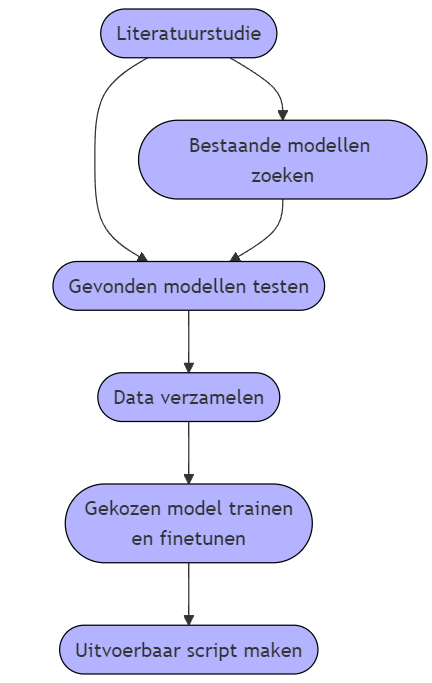
\includegraphics[width=0.6\linewidth]{flow}
\end{center}
Er gebeurde een training met drie verschillende versies van de databank. De eerste training gebeurde aan de hand van fragmenten uit Vlaamse televisieprogramma's. Voor de tweede opzet werd data van het Zorglab toegevoegd in een poging het model te trainen op audio met minder goede kwaliteit en meer ruis. Uiteindelijk werd er voor de derde training teruggekeerd naar de eerste databank, maar gebeurde een herverdeling van de data over de train, test en validatie set.

\section{Resultaten}

Het model gaf na het trainen op de eerste versie van de databank een relatief hoge accuraatheid, maar na het toepassen op de audio van het Zorglab, bleek dit niet het gewenste resultaat te geven. Na de training op de tweede databank was de accuraatheid van het model ongeveer vijf keer lager dan de training op de eerste versie van de databank. Na de derde training was de accuraatheid van het model minder goed dan na de training op de eerste databank, maar er was wel een groter verschil tussen de accuraatheid voor en na het trainen. Onderstaande tabel toont de Diarization Error Rate voor en na elk van de drie trainingen:
\begin{center}
    \captionsetup{type=figure}
    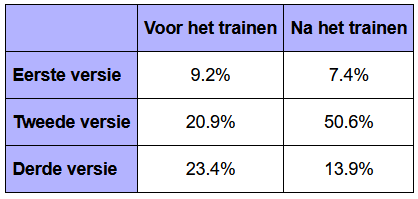
\includegraphics[width=0.6\linewidth]{table}
\end{center}
    
\section{Conclusies}

Het uiteindelijke model was nog niet goed genoeg om te implementeren in de applicatie. Er werd wel gekozen om het model dat getraind werd op de laatste versie van de databank te gebruiken om een uitvoerbaar script te creëren. Dit script kan in verder onderzoek gemakkelijk gebruikt worden en kan zorgen voor een vlottere implementatie van een accurater model.

\section{Toekomstig onderzoek}

Voor toekomstig onderzoek zijn er drie grote mogelijkheden waarvan mogelijks een combinatie gebruikt kan worden:
\begin{itemize}
    \item Ervoor zorgen dat de opnames in het Zorglab betere kwaliteit en minder ruis hebben.
    \item Het trainen uitvoeren op significant grotere hoeveelheid data.
    \item Het model eerst trainen op een databank met enkel duidelijke audio gevolgd door het trainen op een databank met minder kwaliteitsvolle audio.
\end{itemize}

\end{multicols}
\end{document}